\documentclass{beamer}
\usepackage{ctex, hyperref}
\usepackage[T1]{fontenc}
\usepackage{fontspec}
\usefonttheme{serif}              % 使用衬线字体
\usefonttheme{professionalfonts} 
\setmainfont{Times New Roman}
\newfontfamily\chalkd{DejaVu Sans}
\usepackage{latexsym,amsmath,xcolor,multicol,booktabs,calligra}
\usepackage{graphicx,pstricks,listings,stackengine}
% \usepackage{algorithm}
% \usepackage{algorithmic}
\usepackage[ruled, linesnumbered]{algorithm2e}
\usepackage{caption}
\usepackage{float} 
\usepackage{subfigure}

\usepackage[citestyle=authoryear,bibstyle=numeric,sorting=ynt,backend=biber,hyperref=true,backref=true]{biblatex}
\addbibresource{ref.bib}


\author{黄金鸣\quad 郭镇涛}
\title{Managing Weather Risk with a Neural Network-Based Index Insurance}
\subtitle{现代优化方法论文汇报}
\institute{中国人民大学统计学院}
\date{2024年12月17日}
\usepackage{RenminUniv}

% defs
\def\cmd#1{\texttt{\color{red}\footnotesize $\backslash$#1}}
\def\env#1{\texttt{\color{blue}\footnotesize #1}}
\definecolor{deepblue}{rgb}{0,0,0.5}
\definecolor{deepred}{rgb}{0.6,0,0}
\definecolor{deepgreen}{rgb}{0,0.5,0}
\definecolor{halfgray}{gray}{0.55}

\lstset{
    basicstyle=\ttfamily\small,
    keywordstyle=\bfseries\color{deepblue},
    emphstyle=\ttfamily\color{deepred},    % Custom highlighting style
    stringstyle=\color{deepgreen},
    numbers=left,
    numberstyle=\small\color{halfgray},
    rulesepcolor=\color{red!20!green!20!blue!20},
    frame=shadowbox,
}

\begin{document}
\kaishu
\begin{frame}
    \titlepage
    \begin{figure}[htpb]
        \begin{center}
            
\includegraphics[width=0.4\linewidth]{pic/Renmin_Univ_Logo.eps}
        \end{center}
    \end{figure}
\end{frame}

\begin{frame}
    \tableofcontents[sectionstyle=show,subsectionstyle=show/shaded/hide,subsubsectionstyle=show/shaded/hide]
\end{frame}


\section{Introduction}
\begin{frame}[allowframebreaks]{问题背景}
气候变化和天气风险在大规模影响着经济和生计，尤其是依赖于天气条件的农业生产。在实际中，天气指数保险可以用来对冲天气风险。天气指数保险的赔付完全基于一些预设的天气指数而不是受保人实际遭受的损失，因此它避免了传统赔付型保险相关的高行政成本、逆向选择和道德风险问题。

\hfill

尽管前景广阔，但目前的天气指数保险需求较低，这是因为指数保险存在大的基差风险，即基础指数与实际损失之间的不匹配风风险是导致地需求的原因之一。目前大多数指数保险基于低维度天气指数，并使用线性型赔付函数。图(\ref{fig1})显示了基于温度指数的线性保险的赔付情况，显示了较大的基差风险。
\begin{figure}
    \centering
    
    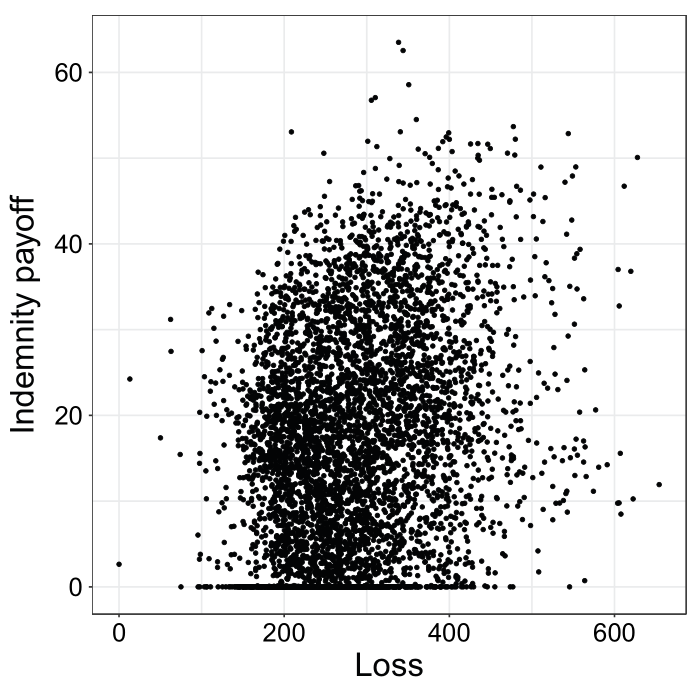
\includegraphics[scale=0.4]{pic/fig1.png}
    \caption{Payoffs of Linear Index Insurance and Actual Losses}
    \label{fig1}
\end{figure}

\cite{2024Chen}旨在通过两方面来减少基差风险。首先，作物生产依赖于高维度的天气指数。因此，在构建保险合同时，应该仔细选择并包含足够多的天气变量；其次，从生物学的角度来看，作物生产队天气条件的依赖时高度非线性的。

\hfill

所以文章提出一种基于神经网络(NN)的指数保险设计。神经网络有助于捕捉天气指数与生产损失之间的高维度、非线性和复杂的相互作用。具体而言，我们将基于神经网络的方案嵌入到一个期望效用最大化问题中，并结合预算约束，以捕捉农民的保险需求。


\end{frame}
\begin{frame}
    
    \begin{figure}[htbp]
        \centering
        \subfigure[]{
        \begin{minipage}[t]{0.3\linewidth}
        \centering
        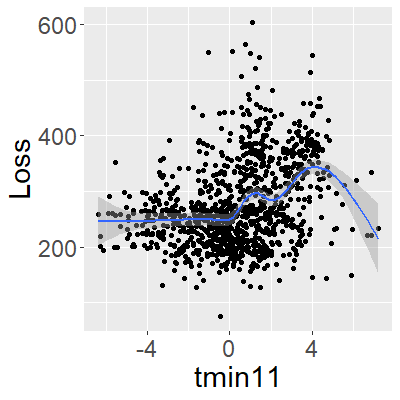
\includegraphics[width=1.2in]{pic/fig2a.png}
        \end{minipage}%
        }%
        \subfigure[]{
        \begin{minipage}[t]{0.3\linewidth}
        \centering
        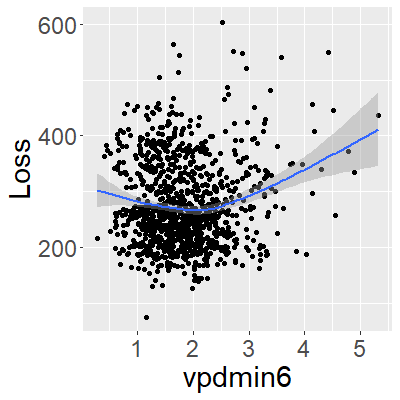
\includegraphics[width=1.2in]{pic/fig2b.png}
        \end{minipage}%
        }%
        \subfigure[]{
        \begin{minipage}[t]{0.3\linewidth}
        \centering
        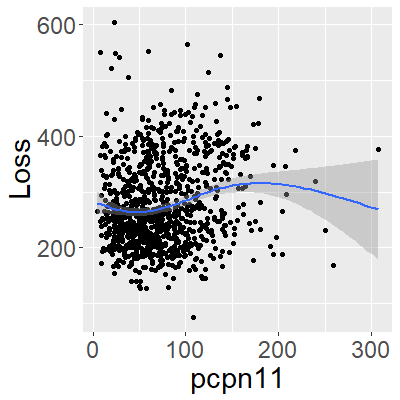
\includegraphics[width=1.2in]{pic/fig2cc.png}
        \end{minipage}
        }%

        \subfigure[]{
        \begin{minipage}[t]{0.3\linewidth}
        \centering
        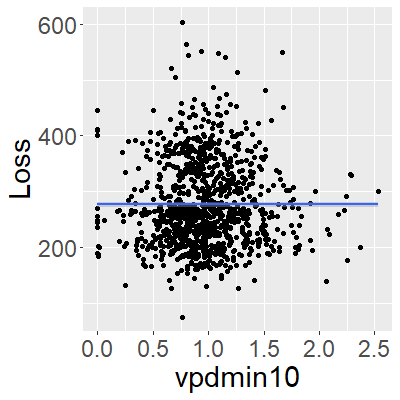
\includegraphics[width=1.2in]{pic/fig2c.png}
        \end{minipage}
        }%
        \subfigure[]{
        \begin{minipage}[t]{0.3\linewidth}
        \centering
        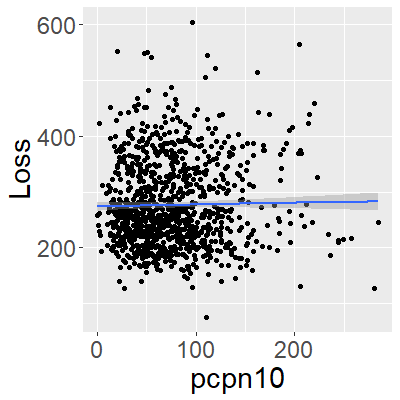
\includegraphics[width=1.2in]{pic/fig2dd.png}
        \end{minipage}
        }%
        \subfigure[]{
        \begin{minipage}[t]{0.3\linewidth}
        \centering
        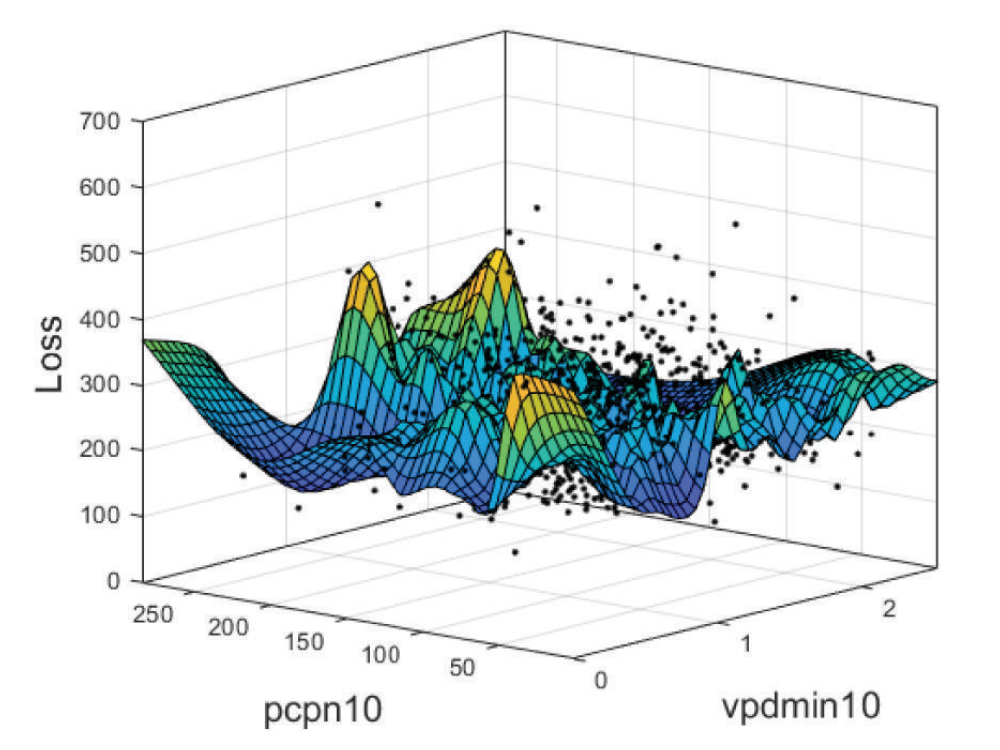
\includegraphics[width=1.3in]{pic/fig2d.png}
        \end{minipage}
        }%
        %\centering
        \caption{Relationship Between Crop Losses and Weather Indices}
    \end{figure}
\end{frame}
\begin{frame}
    我们还测试了基于\texttt{Linear72}模型预测的赔付款，如下图所示：
    \begin{figure}
        \centering
        \caption{Linear72 contract}
        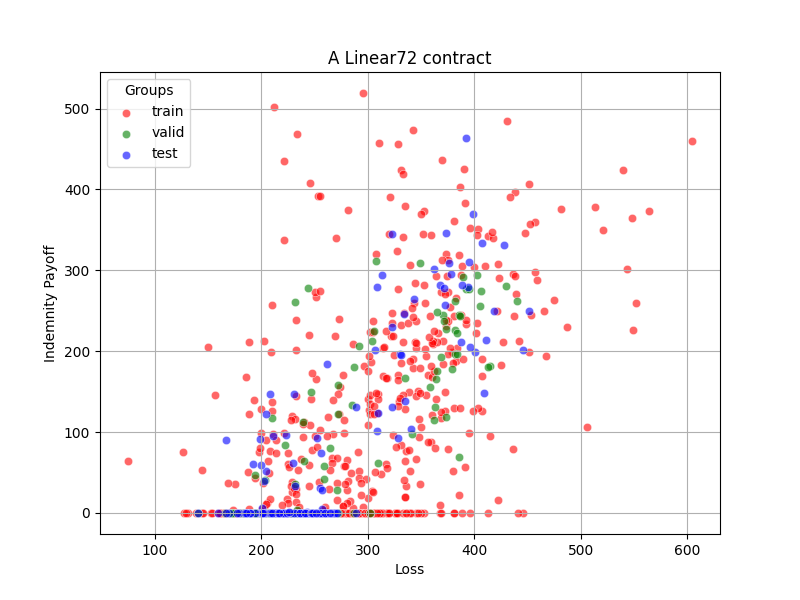
\includegraphics[scale=0.35]{pic/predictionLinear72.png}
    \end{figure}
\end{frame}

\section{Data}
\begin{frame}[allowframebreaks]
    数据方面，关于产量的损失我们采用伊利诺伊州84个县从1925至2018年的数据，我们假设玉米产量损失在去趋势化后在时间和空间上都是同质的，因此我们的样本量大小为7869(84个县$\times$94年-27个缺失数据)；至于天气变量，由于天气的月际变化大而去除特殊年份后不同的年份变化不明显，因此我们选取从1925至2018期间的所有6个天气指标在12个月的数据，即得到一个72维的天气指标矩阵。选取的天气指标如下表所示

    \begin{table}
        \centering
        \caption{天气指数}
        \label{tab1}
        \resizebox{\textwidth}{12mm}{
        \begin{tabular}{ll}
           \hline
           Variable & \multicolumn{1}{c}{Description}  \\
           \hline
           pcpn$k$ & Total precipitation(rain+melted snow)for month $k$ (mm) \\
           tmax$k$ & Daily maximum temperature averaged over all days in month $k$(°C) \\
           tmin$k$ & Daily minimum temperature averaged over all days in month $k$(°C)  \\
           dpt$k$ & Daily mean dew point temperature averaged over all days in month $k$(°C) \\
           vpdmax$k$ & Daily maximum vapor pressure deficit averaged over all days in month $k$ (hPa) \\
           vpnmin$k$ & Daily minimum vapor pressure deficit averaged over all days in month $k$ (hPa) \\
           $k$ & Calendar month, that is, $k=1,2,...,12$ for Jan-Dec\\
           \hline
        \end{tabular}}
        \end{table}
\end{frame}




\section{Model}

\begin{frame}
    本文的指数保险设计问题可以表述为以下的带约束的预期效用最大化问题：
    \begin{equation}
        \left\{
        \begin{aligned}
            \sup_{I\in \mathcal{I}}\quad &\mathbb{E}(U[w_0-Y+I(\boldsymbol{X})-\pi(I)]),\\
            \text{s.t.}\quad &P_L\leq\pi(I)\leq P_\mathcal{U}
        \end{aligned}
        \right. \label{1.1}
    \end{equation}
\end{frame}
\begin{frame}
    其中
    \begin{itemize}
        \item 农民的初始初始财富为$w_0$;
        \item 每年面对的随机生产损失为$Y$;
        \item 指数保险赔付$I(\boldsymbol{X})$由$p$维天气变量$\boldsymbol{X}=(X_1,...,X_p)$决定，其中$I:\mathbb{R}^p\rightarrow\mathbb{R}^+$是一个非负赔付函数；
        \item 指数保险合约的保费(premium)为$\pi(I)$,是赔付函数的一个函数;
        \item 因此，在指数保险存在的情况下，农民的终端财富为$w_0-Y+I(\boldsymbol{X})-\pi(I)$.
    \end{itemize}
    指数保险设计的目标是选择最优的赔付函数$I$,使投保人的预期效用$\mathbb{E}(U)$在一定约束下达到最大化。本文重点针对生产损失的指数保险，不考虑农作物价格风险，即本文考虑的是收益保险。
\end{frame}
\begin{frame}
    我们需要计算预期效用以解决问题$(\ref{1.1})$。但我们并不需要对损失$Y$和天气变量$\boldsymbol{X}$的联合分布进行建模而是用它们的经验分布作为替代并直接寻找最优的指数保险策略。具体来说，对于一个随机样本$(\boldsymbol{X},Y):\{(\boldsymbol{x}_j,y_j)\}_{j=1,...,n},$其中$\boldsymbol{x}_j=(x_{j1},...,x_{jp})$,用样本统计量替换数量后，问题$(\ref{1.1})$可以重写为下面的最小化问题：
    \begin{equation}
        \left\{
        \begin{aligned}
        \min_{I\in\mathcal{I}}\quad&-\frac{1}{n}\sum_{j=1}^n U(w_0-y_j+I(\boldsymbol{x}_j)-\pi_e(I))\\
        \text{s.t.}\quad& P_L\leq \pi_e(I)\leq P_\mathcal{U},
        \end{aligned}
        \right.\label{1.2}
    \end{equation}
    其中$\pi_e(I)$是$\pi(I)$的经验替换，由$\pi_e(I):=(\lambda/n)\sum_{j=1}^nI(\boldsymbol{x_j})$给出。
\end{frame}
\begin{frame}
    考虑一个典型的玉米种植农民，其效用函数为负指数型效用函数$U(w)=-(1/\alpha)e^{-\alpha w},\alpha>0$是绝对风险厌恶系数，在这里我们取$\alpha=0.008$。

    \hfill

    至于保费，本文采用文献和实践中最常用的保费原理来确定指数保险合同的保费，即预期保费原理。即指数保险费$\pi(I)$与期望赔付成比例，如下所示：
    \begin{equation}
        \pi(I)=\lambda\mathbb{E}[I(\boldsymbol{X})],
    \end{equation}
其中$\lambda$是风险载荷参数且$\lambda\geq1$\footnote{文章根据保险合同的供给需求曲线内生地确定均衡$\lambda$,具体步骤如下：首先，通过美国工业部SOB报告的市场数据来拟合供给曲线$Cov=f_S(\lambda),$文章使用历史数据采用非线性最小二乘法将曲线拟合为$\lambda$的幂函数，拟合的供给曲线为$Cov=f_S(\lambda)=7.04\lambda^{2.92}+12.83.$;其次，对于给定$\lambda\in[1.02,1.5]$(这个区间涵盖了指数保险在实际中可行的加载参数)。我们使用基于神经网络的的方法获得对应的最佳指数保险覆盖。通过得到$\lambda$和最佳覆盖的配对数据，我们使用三次Hermite插值多项式拟合需求曲线$Cov=f_D(\lambda)$.最后将供给和需求函数$f_S(\lambda)=f_D(\lambda)$联立求解得出市场均衡下的加载参数$\lambda^*.$}.
\end{frame}
\begin{frame}
\begin{figure}
    \centering
    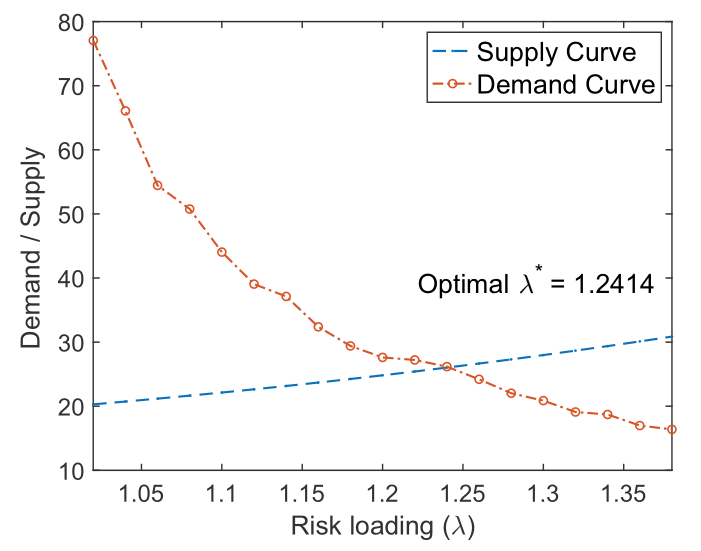
\includegraphics[width=0.7\linewidth]{pic/fig3.png}
    \caption{Supply and Demand Curves of the Index Insurance}
    \label{fig3}
\end{figure}
\end{frame}

\section{NN-Based Solution}
\subsection{Neural Networks and Feasible Set}
\begin{frame}[allowframebreaks]{Feasible Set}
    现有文献和业界通常考虑一个限制性较强的可行集$\tilde{\mathcal{I}}_0\subset \mathcal{I}$,比如阶跃函数（即当某些预定事件发生时触发保险赔付）和分段线性函数（即触发的赔付是指数的线性函数）就是文献中常用的函数形式。然而限制性可行集会导致合同存在较大的基础风险，导致指数保险市场的失败。

\hfill

    本文中我们应用神经网络来寻找在扩展的可行集$\mathcal{I}_0\subset\mathcal{I}$中的最优合同。
    $\mathcal{I}_0$应该足够大，以包含能够捕捉高维度指数与损失之间复杂（非线性、非单调）关系的候选赔付函数，同时$\mathcal{I}_0$也该排除那些在样本数据上非常敏感、无法作为适当保险合同的“表现不稳定”的函数，这样的权衡如图(\ref{fea})所示。

    \begin{figure}
        \centering
        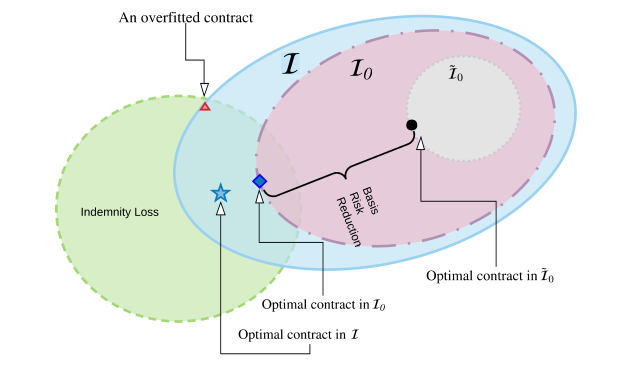
\includegraphics[width=0.9\textwidth]{pic/feasibleset.jpg}
		\caption{Feasible sets and optimal contracts}
        \label{fea}
    \end{figure}
\end{frame}

\begin{frame}{Neural Network}
    我们分别考虑了各种多层的全连接神经网络，其中激活函数使用RELU。经过比较后，我们选择使用一个3层的神经网络（64n16n16n）来作为我们的可行集$\mathcal{I}_0$。
    \begin{figure}
        \centering
        \caption{An illustration of neural networks with $H$-hidden layers}
        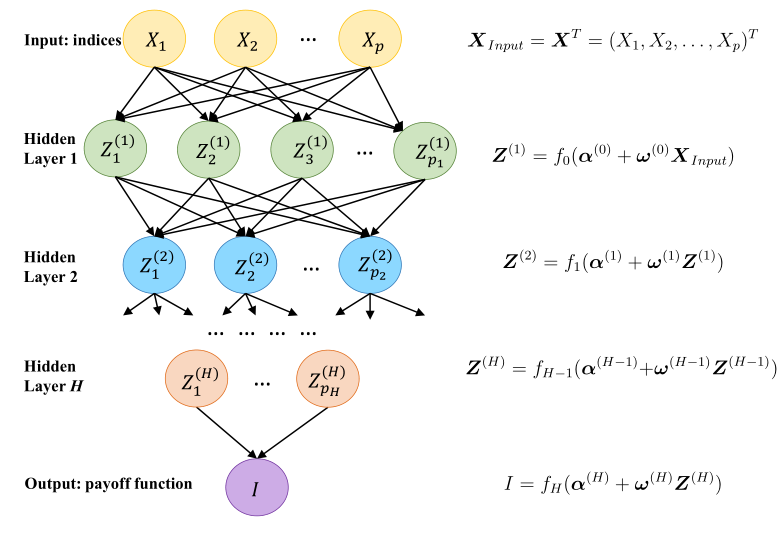
\includegraphics[height=0.5\textheight]{pic/nnetwork.jpg}
    \end{figure}
\end{frame}
\subsection{罚函数法}
\begin{frame}{Solving for the Optimal Policy Using a Penalty Method}
   
    为了解决优化目标存在约束的问题，文章考虑使用罚函数定义一列无约束的问题$\{\Phi_k\}_{k\geq0}$:
    \begin{equation}
        \Phi_k=\min_{I\in \mathcal{I}_0}\Big( -\frac{1}{n}\sum_{j=1}^n U(w-Y_j+I(\boldsymbol{x_j})-\pi_e(I))+\phi_k\cdot g(I) \Big),\label{1.3}
    \end{equation}
    其中$\{\phi_k\}$是一列递增的非负实函数，随着$k$的增大趋向于正无穷，$g(I)$即是惩罚函数。惩罚函数由如下的误差的平方和定义：
    \begin{equation*}
        g(I)=[\max(\pi_e(I)-P_\mathcal{U},0)]^2+[\max(P_L-\pi_e(I),0)]^2.
    \end{equation*}
\end{frame}

\begin{frame}{Solve for the Optimal index insurance policy}
\scalebox{0.72}{
        \begin{algorithm}[H]
        \caption{Solve for the Optimal index insurance policy}\label{alg1}
        \KwOut{An optimal index insurance policy $I$}
        \KwIn{Index data $\boldsymbol{X}$ and loss data $Y$}
        \BlankLine
        Build and initialize a nueral network\;
        Initialization:$k=0,\phi_0=\epsilon_1,\rho>1,$obtain $I$ by solving an unconstrained problem $\Phi_0$\;
        \While{$|I-I_{last}|>\epsilon_3$ \textbf{or}$|\pi_e(I)-\pi_e(I_{last})|>\epsilon_4$}{
            Set $I_{last}=I,\pi_e(I_{last})=\pi_e(I)$\;
            Update $k\gets k+1$,$\phi_{k+1}=\rho\phi_k$\;
            Train the neural network and obtain the optimal $I$ for problem $\Phi_K(I)$:
            \begin{equation*}
                \Phi_k(I) = -\frac{1}{n} \sum_{j=1}^{n} U(w - y_j + I(\boldsymbol{x_j}) - \pi_e(I)) + \phi_k \cdot g(I),
            \end{equation*}
            where the loss function is customized according to $\Phi_k(I)$ and $I_{last}$ is set to the initial value of optimization\;
            Update $g(I)$ and $\pi_e(I)$\;
        }
        \Return{($I$)}\;
        \end{algorithm}
}
\end{frame}
\subsection{增广Lagrange法}
\begin{frame}{Solve for the Optimal Policy using a generalized Lagrange method}
这里我们只有不等式约束，所以令
\begin{equation}
\phi_i(I)=\begin{cases}
-\frac{\lambda_i^2}{2\sigma},&c_i(I)\geq \frac{\lambda_i}{\sigma},\\
\frac{1}{2}\sigma\left[\left(c_i(I) - \frac{\lambda_i}{\sigma}\right)^2-\frac{\lambda_i^2}{\sigma^2}\right],&c_i(I)\leq\frac{\lambda_i}{\sigma},
\end{cases}
\end{equation}
其中\(c_1(I)=\pi_e(I)-P_L\),\(c_2(I)=P_\mathcal{U}-\pi_e(I)\)。
并得到增广Lagrange函数
\[
\Phi(I,\lambda,\sigma)= -\frac{1}{n}\sum_{j=1}^n U(w-Y_j+I(\boldsymbol{x_j})-\pi_e(I))+\sum_i\phi_i(I).
\]
\end{frame}
\begin{frame}{Solve for the Optimal Policy using a generalized Lagrange method}
\scalebox{0.8}{
        \begin{algorithm}[H]
        \caption{Solve for the Optimal index insurance policy}\label{alg2}
        \KwOut{一个最优的指数保险策略$I$}
        \KwIn{天气指数数据 $\boldsymbol{X}$ 以及损失 $Y$}
        \BlankLine
        构造并初始化一个神经网络\;
        初始化：$k=0,\epsilon>0,\lambda_i^0>0,\sigma_0>0,\rho>1$\;
        \While{\([\min\{\pi_e^k(I)-P_L,\frac{\lambda_1^k}{\sigma_k}\}^2+\min\{P_\mathcal{U}-\pi_e^k(I),\frac{\lambda_2^k}{\sigma_k}\}^2]^{1/2}>\epsilon\)}{
            $I_{last}=I$\;
            以$I_{last}$为初始位置训练损失函数为$\Phi(x,\lambda^k,\sigma_k)$的神经网络，并得到此时的最优指数保险$I$\;
            更新\(\lambda^k,\sigma_k\),
            \(\lambda_1^{k+1}=-\sigma_k\min\{\pi_e^k(I)-P_L-\lambda_1^k/\sigma_k, 0\},\)
            \(\lambda_2^{k+1}=-\sigma_k\min\{P_{\mathcal{U}}-\pi_e^k(I)-\lambda_2^k/\sigma_k, 0\},\)
            \(\sigma_{k+1}=\rho\sigma_k\)\;
            \(k\leftarrow k+1\)\;
        }
        \Return{($I$)}\;
        \end{algorithm}
}
\end{frame}
%\section{Optimization Method}
%\begin{frame}{RMSprop}
%    RMSprop(Root Mean Square Propagation)是一种自适应学习率优化器，通过对每个参数的梯度进行平滑处理来调整学习率从而帮助神经网络在训练过程中高效且稳定的收敛。

%    \hfill

%    RMSprop 使用梯度的平方的移动平均来调整每个参数的学习率。具体地说，对于每个参数$θ$，RMSprop 计算其过去一段时间内梯度的平方的指数衰减平均，并使用这个平均值来规范化梯度，从而更新学习率，这意味着梯度较大的参数会有较小的学习率，梯度较小的参数则会有较大的学习率，以期能够在找到某个“凸"结构后快速收敛。

%\end{frame}
%\begin{frame}{RMSprop}
%    \begin{algorithm}[H]
%    \caption{RMSprop Optimization}
%    \KwIn{Initial parameters $\theta$}
%    \KwIn{Learning rate $\epsilon$, decay factor $\rho$}
%    \KwIn{Small constant $\delta$, usually set to $10^{-6}$}
%    \KwOut{Updated parameters $\theta$}
%    \BlankLine
%    Initialize cumulative variables $\boldsymbol{r} = 0$\;
%    \While{Stopping criteria not met}{
%        Take a small batch containing $m$ samples from the training set $\{x^{(1)},...,x^{(m)}\}$, and the corresponding target is $y^{(i)}$\;
%        Compute gradient: $\boldsymbol{g} \gets \frac{1}{m} \nabla_\theta \sum_{i=1}^m L(f(x^{(i)};\theta), y^{(i)})$\;
%        Cumulate squared gradient: $r \gets \rho r + (1 - \rho) \boldsymbol{g} \odot \boldsymbol{g}$\;
%        Compute parameter update: $\Delta \theta = -\frac{\epsilon}{\sqrt{\delta + r}} \odot \boldsymbol{g}$\;
%        Apply the update: $\theta \gets \theta + \Delta \theta$\;
%    }
%    \end{algorithm}
%    \end{frame}


\section{Result}
\begin{frame}[allowframebreaks]{Result with Penalty Method}
    我们考虑以下情况：$w_0=389,P_L=5,P_\mathcal{U}=500$，并且按照时间顺序把前70\%分为训练集，中间15\%被分为验证集，最后15\%被分为测试集。
    先使用罚函数法，罚函数系数$\phi_0=10^{-6}$, $\phi_{k+1}=1.2\phi_k$，并且当$\phi_k\geq0.1$时终止训练，最后结果如下：
    \begin{figure}[htbp]
        \centering
        \subfigure[Rmsprop]{
\includegraphics[width=0.45\textwidth]{pic/penaltyrmsprop.png}}
        \subfigure[Adam]{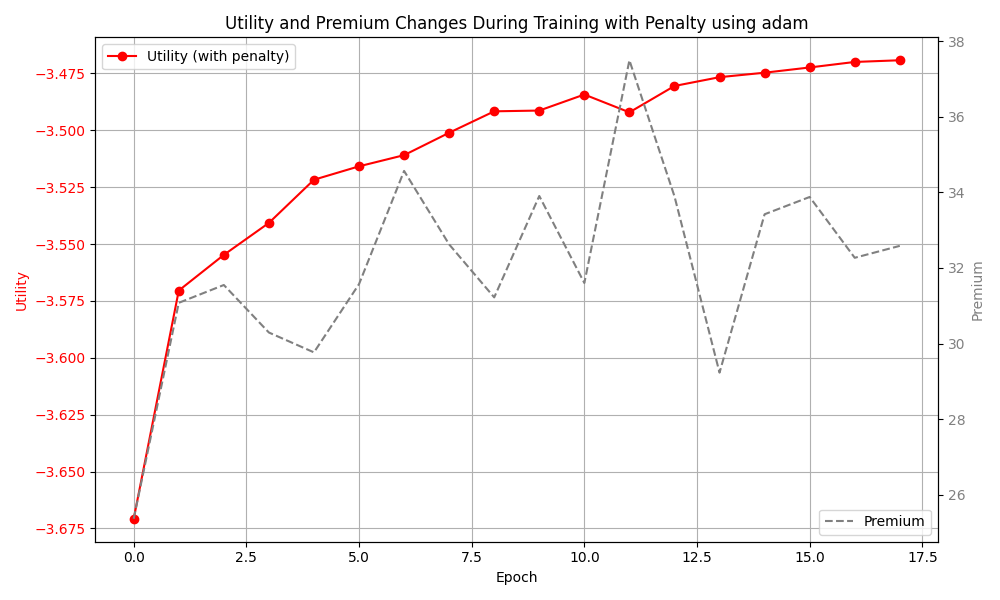
\includegraphics[width=0.45\textwidth]{pic/penaltyadam.png}}
        \caption{Utility and Premium Change During Training with Penalty}
    \end{figure}   


% Table generated by Excel2LaTeX from sheet 'result_penaltyrmsprop'
\begin{table}[htbp]
  \centering
  \caption{Result with Penalty Method using Rmsprop}
    \begin{tabular}{lccc}
    \hline
          & train & valid & test \\
    \hline
    U with insurance & -3.48252 & -3.15697 & -2.99893 \\
    U w/o insurance & -3.87798 & -3.20684 & -3.1225 \\
    U improvement(\%) & 10.1976 & 1.555 & 3.9573 \\
    CEW with insurance & 447.5698 & 459.8376 & 466.2571 \\
    CEW w/o insurance & 434.125 & 457.8786 & 461.21 \\
    CEW improvement & 13.44478 & 1.959049 & 5.047125 \\
    CEW improvement (\%) & 0.03097 & 0.004279 & 0.010943 \\
    Premium & 31.3519 & 16.605 & 16.76953 \\
    \hline
    \end{tabular}%
  \label{tab:penalty rmsprop}%
\end{table}%
% Table generated by Excel2LaTeX from sheet 'result_penaltyadam'
\begin{table}[htbp]
  \centering
  \caption{Result with Penalty Method using Adam}
    \begin{tabular}{lccc}
    \hline
          & train & valid & test \\
    \hline
    U with insurance & -3.46919 & -3.08229 & -2.9239 \\
    U w/o insurance & -3.87798 & -3.20684 & -3.1225 \\
    U improvement(\%) & 10.5413 & 3.8838 & 6.3604 \\
    CEW with insurance & 448.0491 & 462.8301 & 469.4246 \\
    CEW w/o insurance & 434.125 & 457.8786 & 461.21 \\
    CEW improvement & 13.92411 & 4.951489 & 8.214612 \\
    CEW improvement (\%) & 0.032074 & 0.010814 & 0.017811 \\
    Premium & 32.58364 & 15.9892 & 17.72511 \\
    \hline
    \end{tabular}%
  \label{tab:penalty adam}%
\end{table}%


\end{frame}

\begin{frame}[allowframebreaks]{Result with Augmented Lagrange Method}
    除了本文考虑的罚函数方法，我们还使用了增广拉格朗日法，并且参数$\epsilon=10^{-8},\lambda_i^0=2,\sigma=10^{-3},\rho=1.2$。最终结果如下图和下表所示
    \begin{figure}[htbp]
        \centering
        \subfigure[Rmsprop]{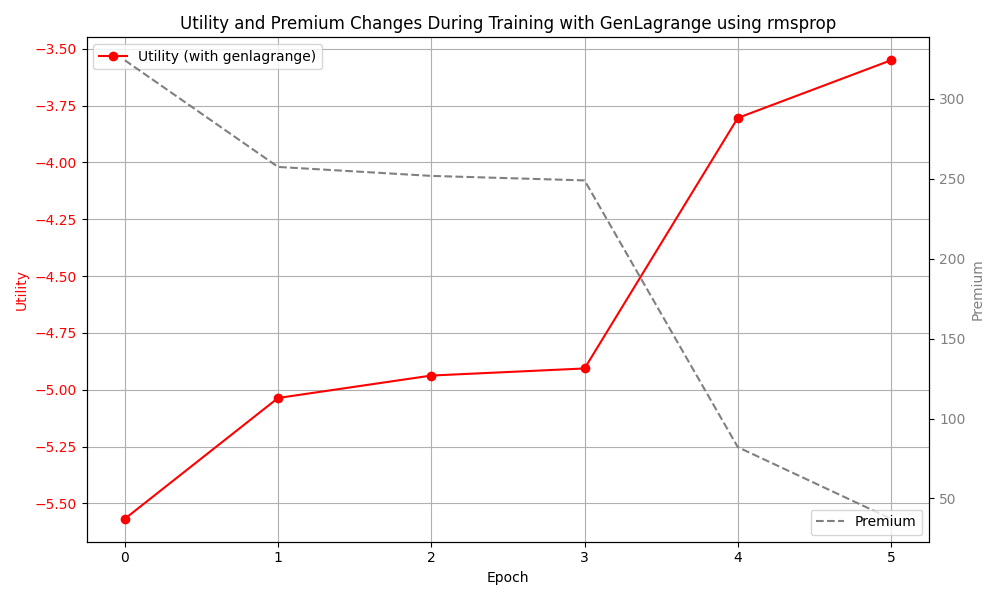
\includegraphics[width=0.45\textwidth]{pic/genLrmsprop.png}}
        \subfigure[Adam]{
\includegraphics[width=0.45\textwidth]{pic/genLadam.png}}
        \caption{Utility and Premium Change During Training with Augmented Lagrange}

    \end{figure}   

% Table generated by Excel2LaTeX from sheet 'result_genlrmsprop'
\begin{table}[htbp]
  \centering
  \caption{Result with generalized Lagrange using Rmsprop}
    \begin{tabular}{lccc}
    \hline
          & train & valid & test \\
    \hline
    U with insurance & -3.55105 & -3.05053 & -2.90317 \\
    U w/o insurance & -3.87798 & -3.20684 & -3.1225 \\
    U improvement(\%) & 8.4302 & 4.8742 & 7.0242 \\
    CEW with insurance & 445.1337 & 464.1249 & 470.3139 \\
    CEW w/o insurance & 434.125 & 457.8786 & 461.21 \\
    CEW improvement & 11.00863 & 6.24629 & 9.10392 \\
    CEW improvement (\%) & 0.025358 & 0.013642 & 0.019739 \\
    Premium & 37.28808 & 36.67967 & 37.03973 \\
    \hline
    \end{tabular}%
  \label{tab:genlrmsprop}%
\end{table}%
% Table generated by Excel2LaTeX from sheet 'result_genladam'
\begin{table}[htbp]
  \centering
  \caption{Result with generalized Lagrange using Adam}
    \begin{tabular}{lccc}
    \hline
          & train & valid & test \\
    \hline
    U with insurance & -3.54797 & -3.03919 & -2.89323 \\
    U w/o insurance & -3.87798 & -3.20684 & -3.1225 \\
    U improvement(\%) & 8.5098 & 5.2278 & 7.3425 \\
    CEW with insurance & 445.2423 & 464.5903 & 470.7425 \\
    CEW w/o insurance & 434.125 & 457.8786 & 461.21 \\
    CEW improvement & 11.11727 & 6.711718 & 9.532487 \\
    CEW improvement (\%) & 0.025608 & 0.014658 & 0.020668 \\
    Premium & 35.74396 & 34.18185 & 34.58889 \\
    \hline
    \end{tabular}%
  \label{tab:gernladam}%
\end{table}%


\end{frame}

\begin{frame}{An optimal NN-based contract}

    \begin{figure}[htbp]
        \centering
        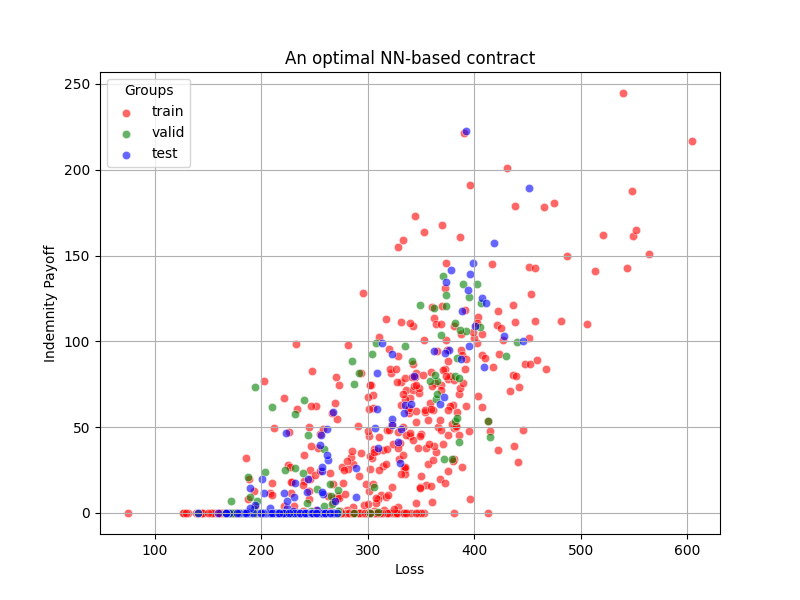
\includegraphics[width=0.9\textwidth]{pic/fig1b1.png}
    \end{figure} 
\end{frame}



% \subsection{如何更好地做Beamer}

% \begin{frame}{Why Beamer}
%     \begin{itemize}
%         \item \LaTeX 广泛用于学术界，期刊会议论文模板
%     \end{itemize}
%     \begin{table}[h]
%         \centering
%         \begin{tabular}{c|c}
%             Microsoft\textsuperscript{\textregistered}  Word & \LaTeX \\
%             \hline
%             文字处理工具 & 专业排版软件 \\
%             容易上手，简单直观 & 容易上手 \\
%             所见即所得 & 所见即所想，所想即所得 \\
%             高级功能不易掌握 & 进阶难，但一般用不到 \\
%             处理长文档需要丰富经验 & 和短文档处理基本无异 \\
%             花费大量时间调格式 & 无需担心格式，专心作者内容 \\
%             公式排版差强人意 & 尤其擅长公式排版 \\
%             二进制格式，兼容性差 & 文本文件，易读、稳定 \\
%             付费商业许可 & 自由免费使用 \\
%         \end{tabular}
%     \end{table}
% \end{frame}

% \begin{frame}{排版举例}
%     \begin{exampleblock}{无编号公式} % 加 * 
%         \begin{equation*}
%             J(\theta) = \mathbb{E}_{\pi_\theta}[G_t] = \sum_{s\in\mathcal{S}} d^\pi (s)V^\pi(s)=\sum_{s\in\mathcal{S}} d^\pi(s)\sum_{a\in\mathcal{A}}\pi_\theta(a|s)Q^\pi(s,a)
%         \end{equation*}
%     \end{exampleblock}
%     \begin{exampleblock}{多行多列公式\footnote{如果公式中有文字出现，请用 $\backslash$mathrm\{\} 或者 $\backslash$text\{\} 包含，不然就会变成 $clip$，在公式里看起来比 $\mathrm{clip}$ 丑非常多。}}
%         % 使用 & 分隔
%         \begin{align}
%             Q_\mathrm{target}&=r+\gamma Q^\pi(s^\prime, \pi_\theta(s^\prime)+\epsilon)\\
%             \epsilon&\sim\mathrm{clip}(\mathcal{N}(0, \sigma), -c, c)\nonumber
%         \end{align}
%     \end{exampleblock}
% \end{frame}

% \begin{frame}
%     \begin{exampleblock}{编号多行公式}
%         % Taken from Mathmode.tex
%         \begin{multline}
%             A=\lim_{n\rightarrow\infty}\Delta x\left(a^{2}+\left(a^{2}+2a\Delta x+\left(\Delta x\right)^{2}\right)\right.\label{eq:reset}\\
%             +\left(a^{2}+2\cdot2a\Delta x+2^{2}\left(\Delta x\right)^{2}\right)\\
%             +\left(a^{2}+2\cdot3a\Delta x+3^{2}\left(\Delta x\right)^{2}\right)\\
%             +\ldots\\
%             \left.+\left(a^{2}+2\cdot(n-1)a\Delta x+(n-1)^{2}\left(\Delta x\right)^{2}\right)\right)\\
%             =\frac{1}{3}\left(b^{3}-a^{3}\right)
%         \end{multline}
%     \end{exampleblock}
% \end{frame}

% \begin{frame}{图形与分栏}
%     % From thuthesis user guide.
%     \begin{minipage}[c]{0.3\linewidth}
%         \psset{unit=0.8cm}
%         \begin{pspicture}(-1.75,-3)(3.25,4)
%             \psline[linewidth=0.25pt](0,0)(0,4)
%             \rput[tl]{0}(0.2,2){$\vec e_z$}
%             \rput[tr]{0}(-0.9,1.4){$\vec e$}
%             \rput[tl]{0}(2.8,-1.1){$\vec C_{ptm{ext}}$}
%             \rput[br]{0}(-0.3,2.1){$\theta$}
%             \rput{25}(0,0){%
%             \psframe[fillstyle=solid,fillcolor=lightgray,linewidth=.8pt](-0.1,-3.2)(0.1,0)}
%             \rput{25}(0,0){%
%             \psellipse[fillstyle=solid,fillcolor=yellow,linewidth=3pt](0,0)(1.5,0.5)}
%             \rput{25}(0,0){%
%             \psframe[fillstyle=solid,fillcolor=lightgray,linewidth=.8pt](-0.1,0)(0.1,3.2)}
%             \rput{25}(0,0){\psline[linecolor=red,linewidth=1.5pt]{->}(0,0)(0.,2)}
% %           \psRotation{0}(0,3.5){$\dot\phi$}
% %           \psRotation{25}(-1.2,2.6){$\dot\psi$}
%             \psline[linecolor=red,linewidth=1.25pt]{->}(0,0)(0,2)
%             \psline[linecolor=red,linewidth=1.25pt]{->}(0,0)(3,-1)
%             \psline[linecolor=red,linewidth=1.25pt]{->}(0,0)(2.85,-0.95)
%             \psarc{->}{2.1}{90}{112.5}
%             \rput[bl](.1,.01){C}
%         \end{pspicture}
%     \end{minipage}\hspace{1cm}
%     \begin{minipage}{0.5\linewidth}
%         \medskip
%         %\hspace{2cm}
%         \begin{figure}[h]
%             \centering
%             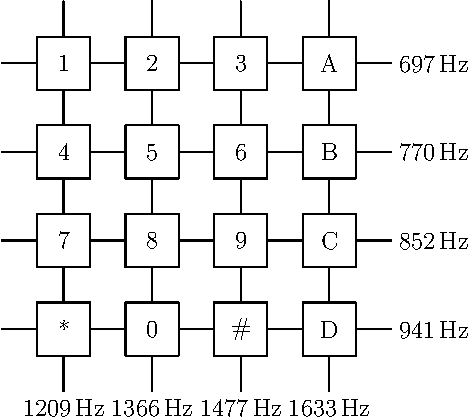
\includegraphics[height=.4\textheight]{pic/dtmf.pdf}
%         \end{figure}
%     \end{minipage}
% \end{frame}

% \begin{frame}[fragile]{\LaTeX{} 常用命令}
%     \begin{exampleblock}{命令}
%         \centering
%         \footnotesize
%         \begin{tabular}{llll}
%             \cmd{chapter} & \cmd{section} & \cmd{subsection} & \cmd{paragraph} \\
%             章 & 节 & 小节 & 带题头段落 \\\hline
%             \cmd{centering} & \cmd{emph} & \cmd{verb} & \cmd{url} \\
%             居中对齐 & 强调 & 原样输出 & 超链接 \\\hline
%             \cmd{footnote} & \cmd{item} & \cmd{caption} & \cmd{includegraphics} \\
%             脚注 & 列表条目 & 标题 & 插入图片 \\\hline
%             \cmd{label} & \cmd{cite} & \cmd{ref} \\
%             标号 & 引用参考文献 & 引用图表公式等\\\hline
%         \end{tabular}
%     \end{exampleblock}
%     \begin{exampleblock}{环境}
%         \centering
%         \footnotesize
%         \begin{tabular}{lll}
%             \env{table} & \env{figure} & \env{equation}\\
%             表格 & 图片 & 公式 \\\hline
%             \env{itemize} & \env{enumerate} & \env{description}\\
%             无编号列表 & 编号列表 & 描述 \\\hline
%         \end{tabular}
%     \end{exampleblock}
% \end{frame}

% \begin{frame}[fragile]{\LaTeX{} 环境命令举例}
%     \begin{minipage}{0.5\linewidth}
% \begin{lstlisting}[language=TeX]
% \begin{itemize}
%   \item A \item B
%   \item C
%   \begin{itemize}
%     \item C-1
%   \end{itemize}
% \end{itemize}
% \end{lstlisting}
%     \end{minipage}\hspace{1cm}
%     \begin{minipage}{0.3\linewidth}
%         \begin{itemize}
%             \item A
%             \item B
%             \item C
%             \begin{itemize}
%                 \item C-1
%             \end{itemize}
%         \end{itemize}
%     \end{minipage}
%     \medskip
%     \pause
%     \begin{minipage}{0.5\linewidth}
% \begin{lstlisting}[language=TeX]
% \begin{enumerate}
%   \item 国民 \item 表率
%   \item 社会
%   \begin{itemize}
%     \item[n+e] 栋梁
%   \end{itemize}
% \end{enumerate}
% \end{lstlisting}
%     \end{minipage}\hspace{1cm}
%     \begin{minipage}{0.3\linewidth}
%         \begin{enumerate}
%             \item 国民
%             \item 表率
%             \item 社会
%             \begin{itemize}
%                 \item[n+e] 栋梁
%             \end{itemize}
%         \end{enumerate}
%     \end{minipage}
% \end{frame}

% \begin{frame}[fragile]{\LaTeX{} 数学公式}
%     \begin{columns}
%         \begin{column}{.55\textwidth}
% \begin{lstlisting}[language=TeX]
% $V = \frac{4}{3}\pi r^3$

% \[
%   V = \frac{4}{3}\pi r^3
% \]

% \begin{equation}
%   \label{eq:vsphere}
%   V = \frac{4}{3}\pi r^3
% \end{equation}
% \end{lstlisting}
%         \end{column}
%         \begin{column}{.4\textwidth}
%             $V = \frac{4}{3}\pi r^3$
%             \[
%                 V = \frac{4}{3}\pi r^3
%             \]
%             \begin{equation}
%                 \label{eq:vsphere}
%                 V = \frac{4}{3}\pi r^3
%             \end{equation}
%         \end{column}
%     \end{columns}
%     \begin{itemize}
%         \item 更多内容请看 \href{https://zh.wikipedia.org/wiki/Help:数学公式}{\color{purple}{这里}}
%     \end{itemize}
% \end{frame}

% \begin{frame}[fragile]
%     \begin{columns}
%         \column{.6\textwidth}
% \begin{lstlisting}[language=TeX]
%     \begin{table}[htbp]
%       \caption{编号与含义}
%       \label{tab:number}
%       \centering
%       \begin{tabular}{cl}
%         \toprule
%         编号 & 含义 \\
%         \midrule
%         1 & 4.0 \\
%         2 & 3.7 \\
%         \bottomrule
%       \end{tabular}
%     \end{table}
%     公式~(\ref{eq:vsphere}) 的
%     编号与含义请参见
%     表~\ref{tab:number}。
% \end{lstlisting}
%         \column{.4\textwidth}
%         \begin{table}[htpb]
%             \centering
%             \caption{编号与含义}
%             \label{tab:number}
%             \begin{tabular}{cl}\toprule
%                 编号 & 含义 \\\midrule
%                 1 & 4.0\\
%                 2 & 3.7\\\bottomrule
%             \end{tabular}
%         \end{table}
%         \normalsize 公式~(\ref{eq:vsphere})的编号与含义请参见表~\ref{tab:number}。
%     \end{columns}
% \end{frame}

% \begin{frame}{作图}
%     \begin{itemize}
%         \item 矢量图 eps, ps, pdf
%         \begin{itemize}
%             \item METAPOST, pstricks, pgf $\ldots$
%             \item Xfig, Dia, Visio, Inkscape $\ldots$
%             \item Matlab / Excel 等保存为 pdf
%         \end{itemize}
%         \item 标量图 png, jpg, tiff $\ldots$
%         \begin{itemize}
%             \item 提高清晰度，避免发虚
%             \item 应尽量避免使用
%         \end{itemize}
%     \end{itemize}
%     \begin{figure}[htpb]
%         \centering
%         
\includegraphics[width=0.2\linewidth]{pic/Renmin_Univ_Logo.eps}
%         \caption{这个校徽就是矢量图}
%     \end{figure}
% \end{frame}

% \section{计划进度}
% \begin{frame}
%     \begin{itemize}
%         \item 一月：完成文献调研
%         \item 二月：复现并评测各种Beamer主题美观程度
%         \item 三、四月：美化THU Beamer主题
%         \item 五月：论文撰写
%     \end{itemize}
% \end{frame}

% \section{参考文献}

\AtEndDocument{
\begin{frame}[allowframebreaks]{}
  \printbibliography
  \nocite{*}
\end{frame}
\begin{frame}
    \begin{center}
        {\Huge\calligra Thanks!}
    \end{center}
\end{frame}
}



\end{document}